\section{Linear Sodium Chain --- Transport properties}
\label{sec14:nachain}

\begin{itemize}
\item Outline: {\it Compare the quantum conductance of a periodic linear chain of Sodium atoms with that
of a defected chain}
\end{itemize}


\begin{figure}[h!]
\centering
\subfloat[periodic]{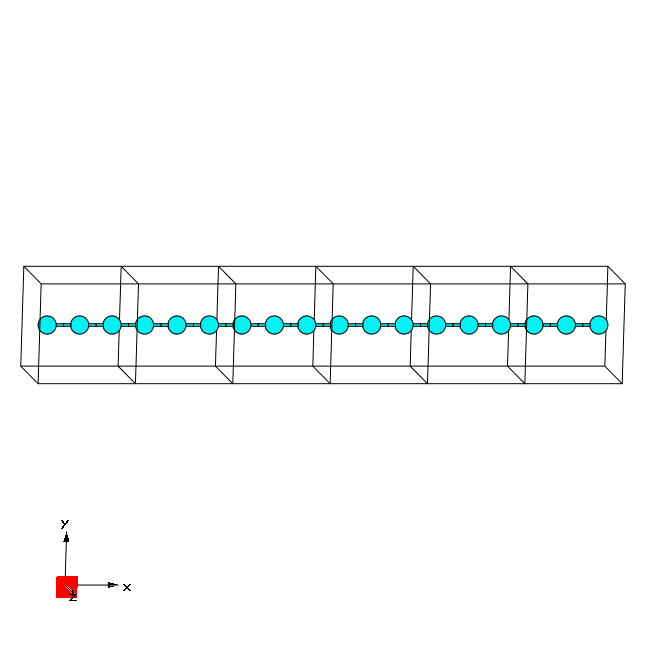
\includegraphics[width=0.7\columnwidth,trim={0pt 200pt 0pt 200pt},clip]{figure/example14/Na_chain.png}}\\
\centering
\subfloat[defected]{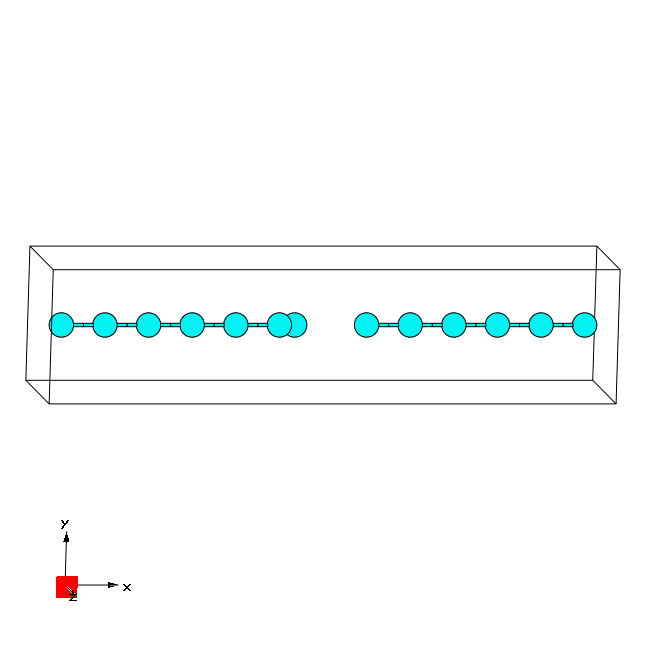
\includegraphics[width=0.7\columnwidth,trim={0pt 200pt 0pt 200pt},clip]{figure/example14/Na_13chain.png}}
\label{fig14.1}
\caption{Unit cell of a periodic linear Sodium chain (left panel) and of a defected linear Sodium chain (right panel) plotted with the \xcrysden{} program. The former consists of 2 Na atom per unit cell (6 unit cells have been drawn for comparison with the defected system). The latter consists of 13 Na atoms per unit cell.}
\end{figure}

\begin{enumerate}
\item [1-2] {\it Run pwscf and wannier90 for the periodic and defected systems.}

\item[3] {\it Compare the quantum conductance of the periodic (bulk) calculation with the defected (LCR) calculation.}

The quantum conductance and the DOS are shown in \Fig{fig14.2}. 

\begin{figure}[b!]
\centering
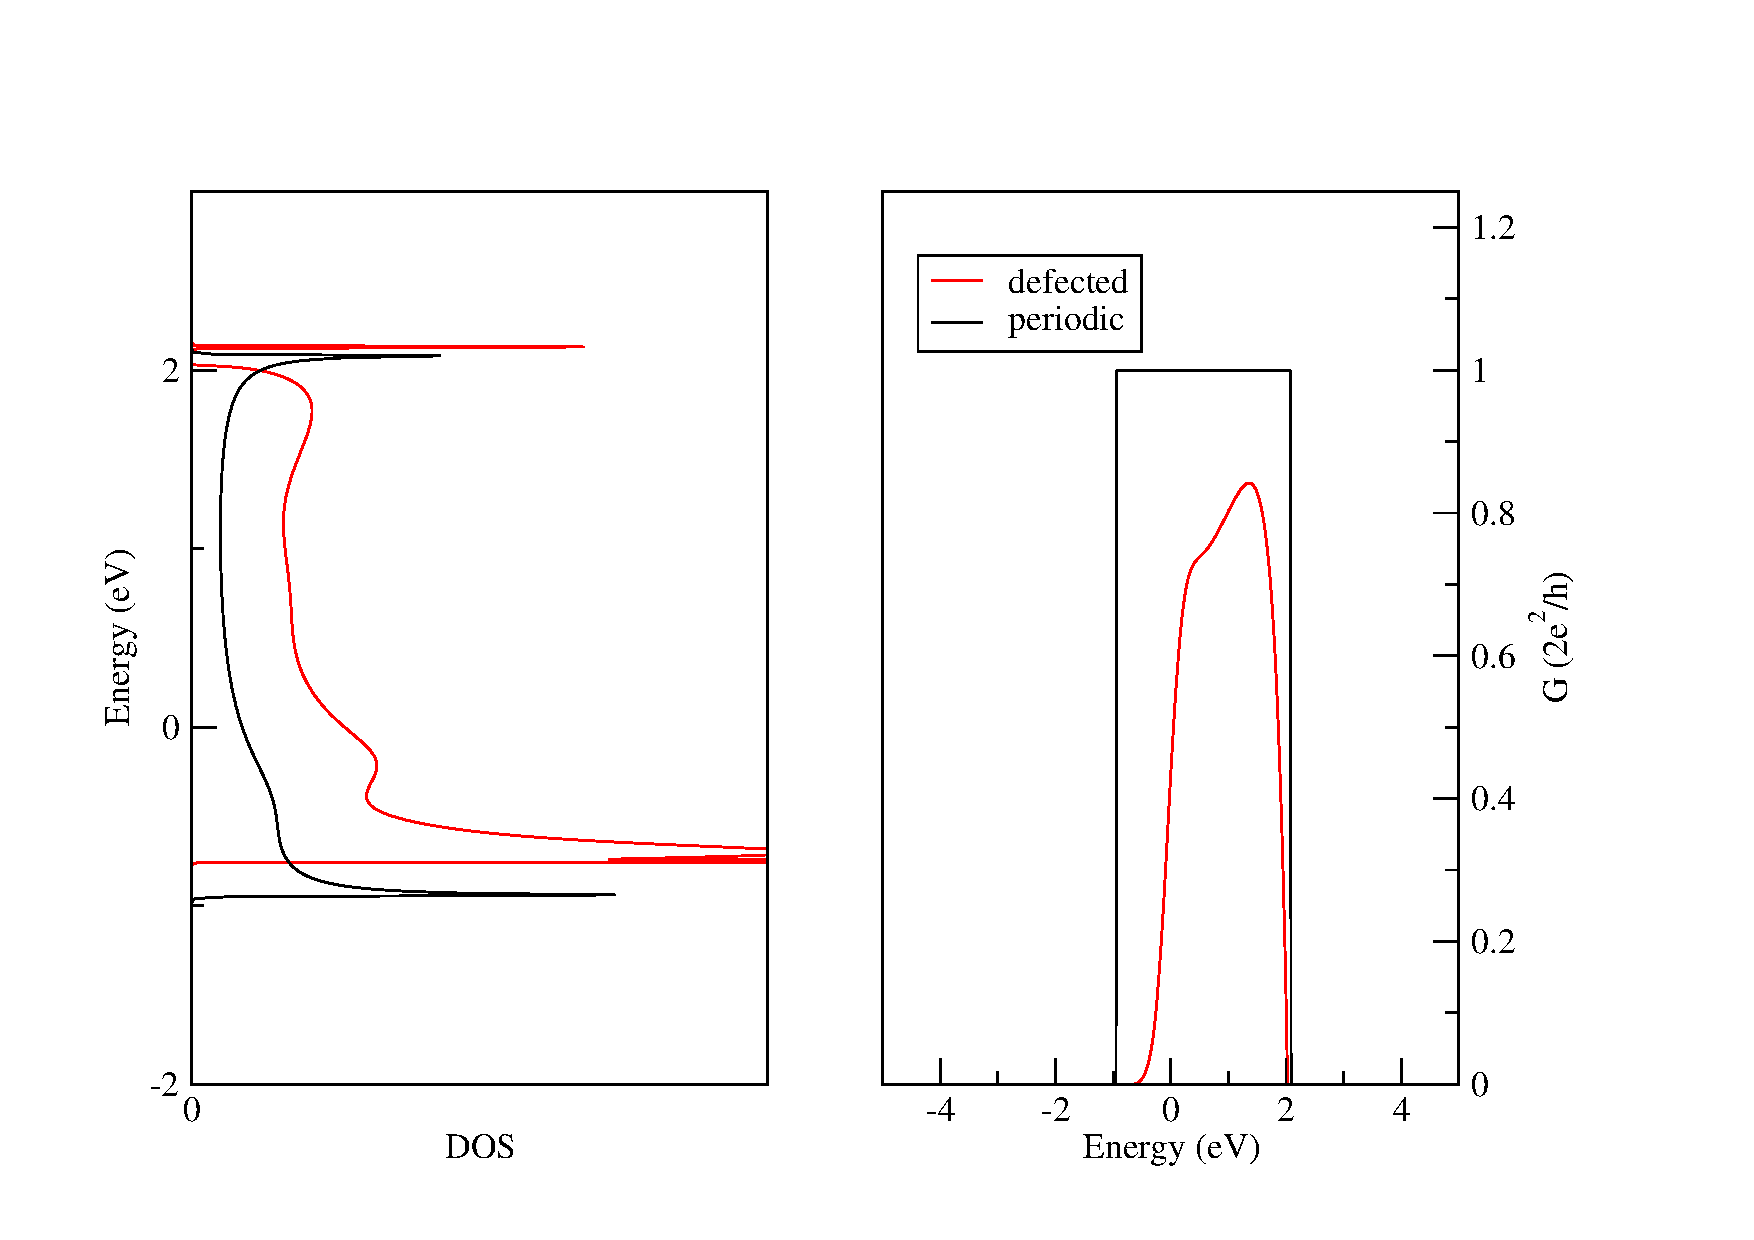
\includegraphics[width=1.0\columnwidth,height=0.5\columnwidth,trim={20pt 10pt 50pt 50pt},clip]{figure/example14/Na_chain_dos_qc.pdf}
\caption{DOS (left) and quantum conductance (right) of periodic (solid black) and defected (solid red) Sodium linear chain.}\label{fig14.2}
\end{figure}
\end{enumerate}
